\documentclass[journal]{vgtc}                % final (journal style)
%\documentclass[review,journal]{vgtc}         % review (journal style)
%\documentclass[widereview]{vgtc}             % wide-spaced review
%\documentclass[preprint,journal]{vgtc}       % preprint (journal style)
%\documentclass[electronic,journal]{vgtc}     % electronic version, journal

%% Uncomment one of the lines above depending on where your paper is
%% in the conference process. ``review'' and ``widereview'' are for review
%% submission, ``preprint'' is for pre-publication, and the final version
%% doesn't use a specific qualifier. Further, ``electronic'' includes
%% hyperreferences for more convenient online viewing.

%% Please use one of the ``review'' options in combination with the
%% assigned online id (see below) ONLY if your paper uses a double blind
%% review process. Some conferences, like IEEE Vis and InfoVis, have NOT
%% in the past.

%% Please note that the use of figures other than the optional teaser is not permitted on the first page
%% of the journal version.  Figures should begin on the second page and be
%% in CMYK or Grey scale format, otherwise, colour shifting may occur
%% during the printing process.  Papers submitted with figures other than the optional teaser on the
%% first page will be refused.

%% These three lines bring in essential packages: ``mathptmx'' for Type 1
%% typefaces, ``graphicx'' for inclusion of EPS figures. and ``times''
%% for proper handling of the times font family.

\usepackage{mathptmx}
\usepackage{graphicx}
\usepackage{times}

%% We encourage the use of mathptmx for consistent usage of times font
%% throughout the proceedings. However, if you encounter conflicts
%% with other math-related packages, you may want to disable it.

%% This turns references into clickable hyperlinks.
\usepackage[bookmarks,backref=true,linkcolor=black]{hyperref} %,colorlinks
\hypersetup{
  pdfauthor = {},
  pdftitle = {},
  pdfsubject = {},
  pdfkeywords = {},
  colorlinks=true,
  linkcolor= black,
  citecolor= black,
  pageanchor=true,
  urlcolor = black,
  plainpages = false,
  linktocpage
}

%% If you are submitting a paper to a conference for review with a double
%% blind reviewing process, please replace the value ``0'' below with your
%% OnlineID. Otherwise, you may safely leave it at ``0''.
\onlineid{0}

%% declare the category of your paper, only shown in review mode
\vgtccategory{Research}

%% allow for this line if you want the electronic option to work properly
\vgtcinsertpkg

%% In preprint mode you may define your own headline.
%\preprinttext{To appear in an IEEE VGTC sponsored conference.}

%% Paper title.

\title{Exploring High Dimensional Data Through\\ Locally Optimized Viewpoint Selection}

%% This is how authors are specified in the journal style

%% indicate IEEE Member or Student Member in form indicated below
%%\author{Roy G. Biv, Ed Grimley, \textit{Member, IEEE}, and Martha Stewart}
%%\authorfooter{
%% insert punctuation at end of each item
%%\item
 %%Roy G. Biv is with Starbucks Research. E-mail: roy.g.biv@aol.com.
%%\item
%% Ed Grimley is with Grimley Widgets, Inc.. E-mail: ed.grimley@aol.com.
%%\item
%% Martha Stewart is with Martha Stewart Enterprises at Microsoft
%% Research. E-mail: martha.stewart@marthastewart.com.
%%}

%other entries to be set up for journal
%% \shortauthortitle{Biv \MakeLowercase{\textit{et al.}}: Global Illumination for Fun and Profit}
%\shortauthortitle{Firstauthor \MakeLowercase{\textit{et al.}}: Paper Title}

%% Abstract section.
\abstract{Dimension reduced projection is usually obtained via a global optimization. It gives a good overview of the data, but cannot satisfy different users with different focuses. That's because any local data could be distorted and misleading due to projection errors. To address this problem, we propose an interactive visualization method, to customize projections for better local analysis. First, we allow users to define their point of interest (POI) data. Then we generate local projections to minimize distortions regarding the POI. Multipe optimizations are provided for different analyses. We also reveal relationships among different POIs, by comparing their local projections. At last, our method is proved effective via case studies with a real-world dataset.
} % end of abstract

%% Keywords that describe your work. Will show as 'Index Terms' in journal
%% please capitalize first letter and insert punctuation after last keyword
\keywords{Dimension-reduced projection, local analysis, high-dimensional data}

%% ACM Computing Classification System (CCS).
%% See <http://www.acm.org/class/1998/> for details.
%% The ``\CCScat'' command takes four arguments.

\CCScatlist{ % not used in journal version
 \CCScat{K.6.1}{Management of Computing and Information Systems}%
{Project and People Management}{Life Cycle};
 \CCScat{K.7.m}{The Computing Profession}{Miscellaneous}{Ethics}
}

%% Uncomment below to include a teaser figure.
  \teaser{
 \centering
 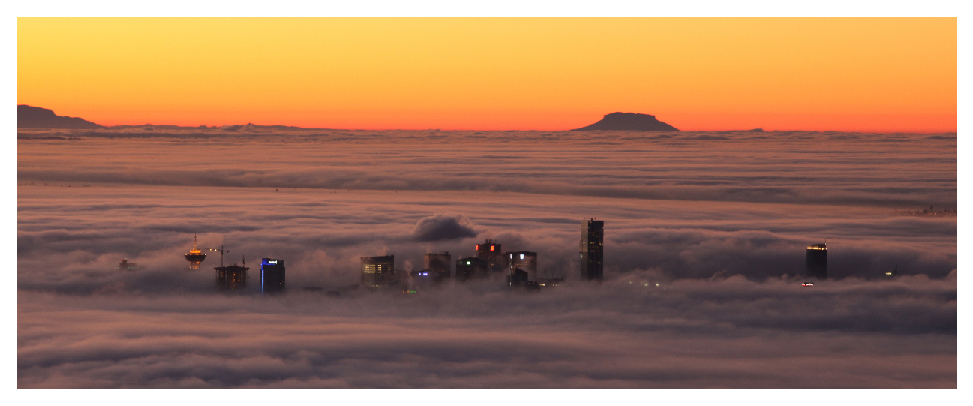
\includegraphics[width=16cm]{CypressView}
  \caption{Teaser here.}
  }

%% Uncomment below to disable the manuscript note
%\renewcommand{\manuscriptnotetxt}{}

%% Copyright space is enabled by default as required by guidelines.
%% It is disabled by the 'review' option or via the following command:
% \nocopyrightspace

%%%%%%%%%%%%%%%%%%%%%%%%%%%%%%%%%%%%%%%%%%%%%%%%%%%%%%%%%%%%%%%%
%%%%%%%%%%%%%%%%%%%%%% START OF THE PAPER %%%%%%%%%%%%%%%%%%%%%%
%%%%%%%%%%%%%%%%%%%%%%%%%%%%%%%%%%%%%%%%%%%%%%%%%%%%%%%%%%%%%%%%%

\begin{document}

%% The ``\maketitle'' command must be the first command after the
%% ``\begin{document}'' command. It prepares and prints the title block.

%% the only exception to this rule is the \firstsection command

%% \section{Introduction} %for journal use above \firstsection{..} instead
\firstsection{Introduction}
\maketitle
Dimension-reduced projection is widely used for high-dimensional data analysis. It seeks to approximate the original distribution in a low-dimensional space. Such approximation is often globally optimized to make a good overview of the data. But due to approximation errors, data relationships will inevitably be distorted. The distortions are hard to ignore when it comes to local data. They largely harm the perception of local structures, yet are often transparent to users. Even if distortions are shown in the projection~\cite{DBLP:journals/tvcg/StahnkeDMT16}~\cite{DBLP:journals/ijon/Aupetit07}, users have no means to control their distribution. In general, globally optimized projections make good overviews, but are not suitable for local data analysis.
%change citation here.

One way to alleviate this problem, is to observe the data in a different perspective. Some previous works~\cite{DBLP:journals/cgf/JeongZFRC09}~\cite{DBLP:journals/tvcg/NamM13}~\cite{DBLP:journals/tvcg/LehmannT13} allow users to change the projection by adjusting dimension weights. It helps to clarify detailed structures and find out more useful information. To help build a targeted analysis, featured clusters are often provided beforehand~\cite{DBLP:journals/tvcg/NamM13}~\cite{DBLP:journals/cgf/LiuWTBP15}. However, users know nothing about the given clusters. They have to solve their puzzles by manually searching the enormous data space. It's a blinded and exhausting process, where users have no clue how to steer the dimensions to get a better view. Even if interesting projections are found, it's hard to explain or assess them without distortion information.

Compared to dimension-based exploration, feature-based mining techniques are more efficient in revealing informative projections. Projection pursuit~\cite{DBLP:journals/tc/FriedmanT74} searches for projections to optimize predefined indices. The rank-by-feature framework~\cite{DBLP:journals/ivs/SeoS05} ranks a series of projections by their interestingness. In more recent works, users are involved to specify desired features~\cite{DBLP:journals/tvcg/JohanssonJ09} and relationships~\cite{DBLP:journals/tvcg/HuBMHNL13}~\cite{DBLP:journals/tvcg/Gleicher13}. These methods, though effective, largely depend on predefined metrics or users' prior knowledge. It makes them unsuitable for an interactive exploration starting from scratch. Besides, little attention had been paid to facilitate local data analysis.

In this work, we propose an interactive exploration method, that promotes consecutive local data analyses in locally optimized projections.

\note{
Nevertheless, local analysis is not only necessary, but also an efficient way to explore high-dimensional data. On one hand, a sole overview cannot show all aspects.\note{especially when the dimensionality is high.} After a quick glance, users tend to pick up some local structure (e.g. clusters, outliers) and go into details. It helps them fully understand the data and discover more useful information. On the other hand, featured local data are good breakthrough points for an efficient exploration. Traditional methods~\cite{DBLP:journals/tvcg/NamM13}~\cite{DBLP:journals/tvcg/LehmannT13} allow users to change the projection by adjusting dimensions. But such exploration is blind and exhausting, since the data space is huge while users have no clue where to go. Compared to dimensions, data features are easier to perceive and explain. That's why dimension-based explorations often provide featured clusters as start points~\cite{DBLP:journals/tvcg/NamM13}~\cite{DBLP:journals/cgf/LiuWTBP15}. It's also the spirit behind feature-based projection mining techniques, such as projection pursuit~\cite{DBLP:journals/tc/FriedmanT74} and the rank-by-feature framework~\cite{DBLP:journals/ivs/SeoS05}.
}
\section{Related Work}
\label{section:relatedwork}

\subsection{Dimension-Driven Projection Exploration}
\textbf{Dimension Manipulation and Grand Tour}
~\cite{DBLP:journals/tvcg/NamM13}~\cite{DBLP:journals/tvcg/LehmannT13}~\cite{DBLP:journals/cgf/JeongZFRC09}
%Define principle component analysis (PCA)

\subsection{Data-Driven Projection Pursuit}
\textbf{Projection Pursuit}
~\cite{DBLP:journals/tc/FriedmanT74}~\cite{cook1995grand}~\cite{DBLP:journals/ivs/SeoS05}~\cite{DBLP:journals/tvcg/JohanssonJ09}~\cite{DBLP:conf/apvis/NhonW14}

\textbf{Projection Pursuit for Classification}
~\cite{DBLP:journals/cgf/SipsNLH09}~\cite{DBLP:conf/ieeevast/ChooLKP10}~\cite{DBLP:conf/ieeevast/TatuAESTMK09}~\cite{DBLP:journals/cgf/SedlmairTMT12}~\cite{DBLP:conf/ieeevast/AlbuquerqueEM11}

\textbf{Targeted Projection Pursuit}
~\cite{DBLP:journals/tvcg/JoiaCCPN11}~\cite{DBLP:conf/ieeevast/BrownLBC12}~\cite{DBLP:journals/tvcg/Gleicher13}~\cite{DBLP:journals/tvcg/HuBMHNL13}

\subsection{High-Dimensional Local Data Analysis}
\textbf{Distortion Analysis}
~\cite{DBLP:journals/cg/MartinsCMT14}~\cite{DBLP:journals/cgf/LiuWBP14}~\cite{DBLP:journals/tvcg/StahnkeDMT16}

\textbf{Subspace Cluster Estimation}
~\cite{DBLP:conf/ieeevast/NamHMZI07}~\cite{DBLP:journals/tsp/CarterRH10}~\cite{DBLP:conf/ieeevast/Kandogan12}~\cite{DBLP:journals/tvcg/YuanRWG13}~\cite{DBLP:journals/cgf/LiuWTBP15}
\section{Overview}

\ifx
\begin{figure*}[htb]
\centering
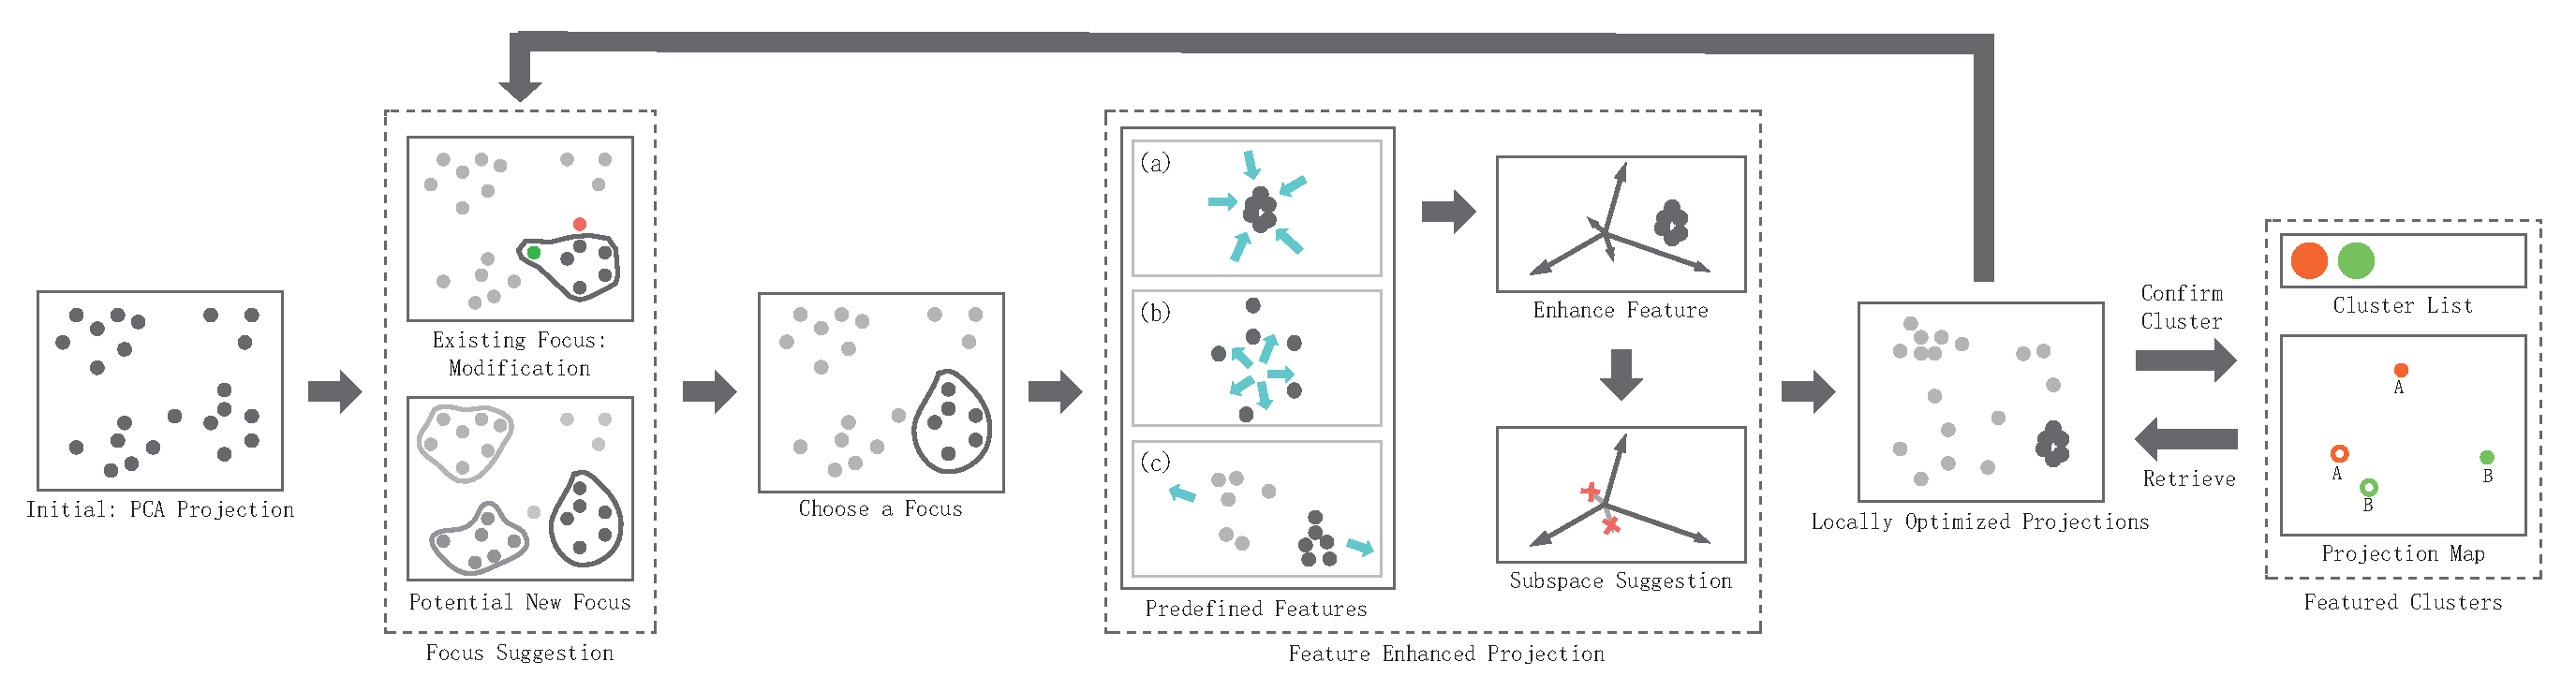
\includegraphics{images/Pipeline.eps}
\caption{Sample illustration.}
\end{figure*}
\else
\begin{figure*}[htbp]
\centering
  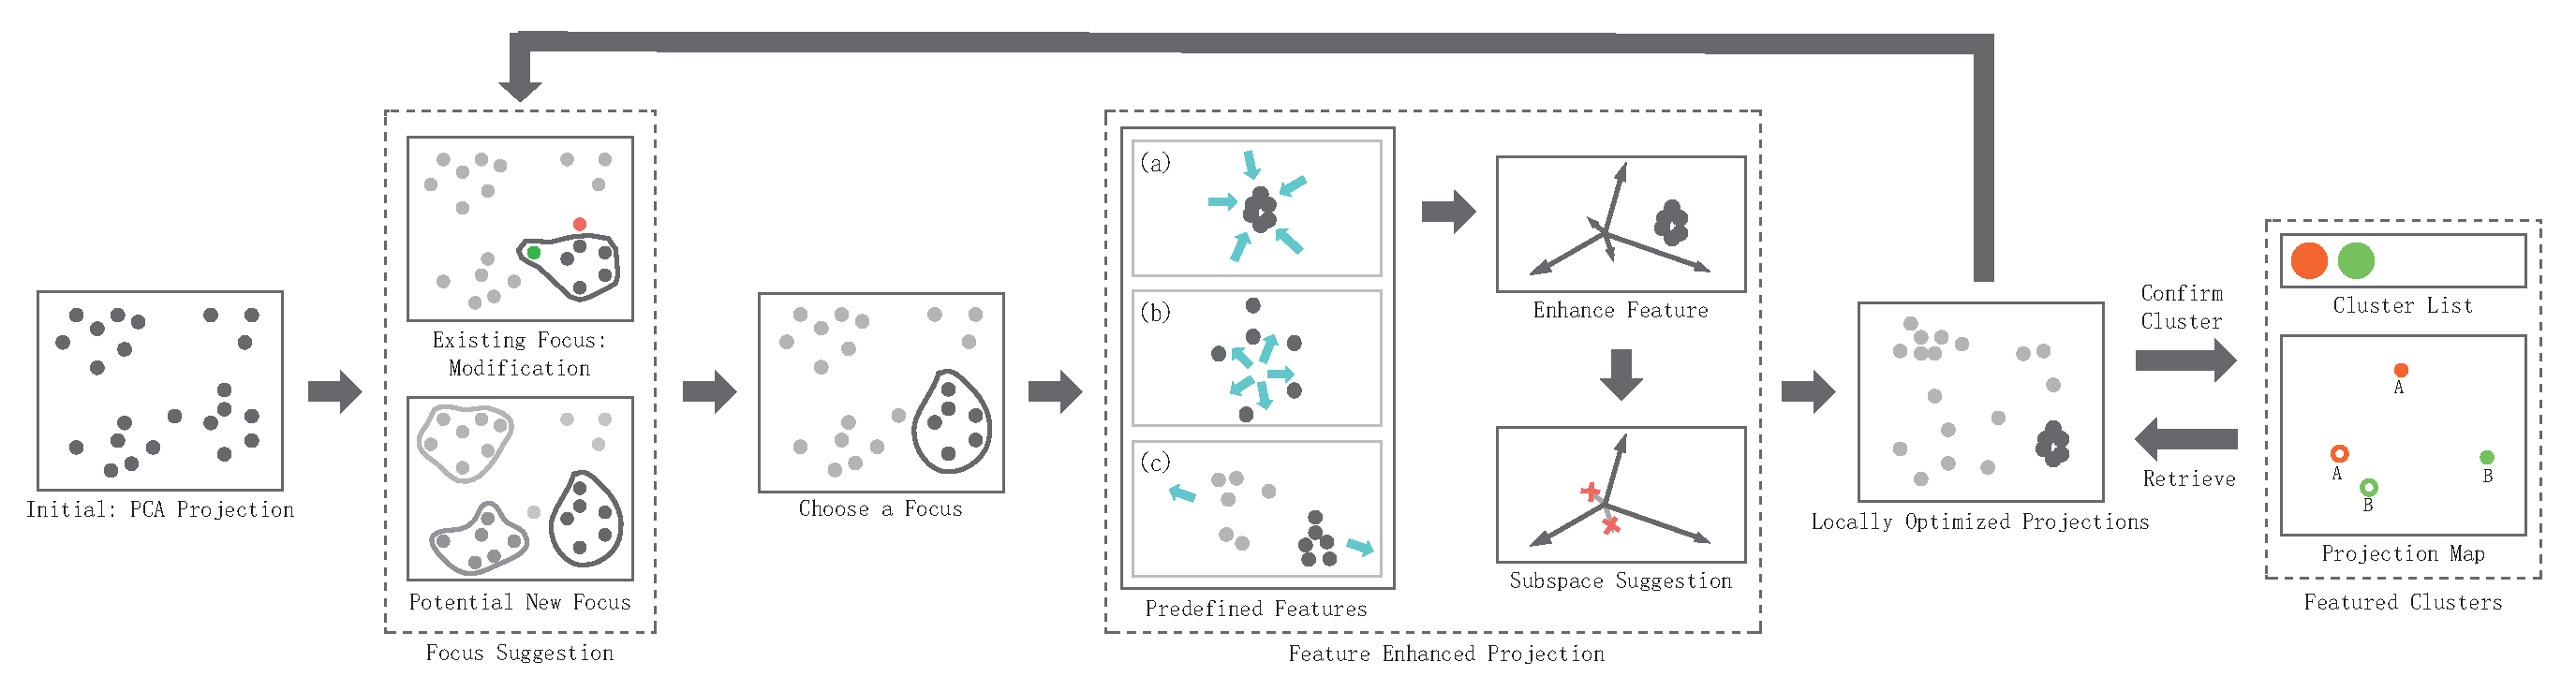
\includegraphics[width=1\linewidth]{images/Pipeline.eps}% 1\linewidth
  \caption{The overview of delivery system.}\label{fig.2}
  \end{figure*}
  \fi

\section{Locally Optimized Viewpoint Selection}

Lorem ipsum dolor sit amet, consetetur sadipscing elitr, sed diam
nonumy eirmod tempor invidunt ut labore et dolore magna aliquyam erat,
sed diam voluptua. At vero eos et accusam et justo duo dolores et ea
rebum. Stet clita kasd gubergren, no sea takimata sanctus est Lorem
ipsum dolor sit amet. Lorem ipsum dolor sit amet, consetetur
sadipscing elitr, sed diam nonumy eirmod tempor invidunt ut labore et
dolore magna aliquyam erat, sed diam voluptua. At vero eos et accusam
et justo duo dolores et ea rebum. Stet clita kasd gubergren, no sea
takimata sanctus est Lorem ipsum dolor sit amet. Lorem ipsum dolor sit
amet, consetetur sadipscing elitr, sed diam nonumy eirmod tempor
invidunt ut labore et dolore magna aliquyam erat, sed diam
voluptua. At vero eos et accusam et justo duo dolores et ea
rebum. Stet clita kasd gubergren, no sea takimata sanctus est Lorem
ipsum dolor sit amet.

Lorem ipsum dolor sit amet, consetetur sadipscing elitr, sed diam
nonumy eirmod tempor invidunt ut labore et dolore magna aliquyam erat,
sed diam voluptua. At vero eos et accusam et justo duo dolores et ea
rebum. Stet clita kasd gubergren, no sea takimata sanctus est Lorem
ipsum dolor sit amet. Lorem ipsum dolor sit amet, consetetur
sadipscing elitr, sed diam nonumy eirmod tempor invidunt ut labore et
dolore magna aliquyam erat, sed diam voluptua. At vero eos et accusam
et justo duo dolores et ea rebum.

\section{Case Study}
\label{section:casestudy}
In this section, we demonstrate the effectiveness of our method with two real-world datasets.

\subsection{Cars Data}
\label{case:car}
For the first case, we present a neighborhood study on the Cars dataset~\cite{Lichman:2013}. The dataset contains 392 cars with 8 attributes: displacement, MPG, cylinder number, horsepower, weight, acceleration time, year and origin.

\begin{figure}[htbp]
\centering
  \includegraphics[width=0.7\linewidth]{images/car_1.eps}% 1\linewidth
  \caption{Car Data: In the global projection~(a), we find a misplaced datum with the help of focus point suggestion~(b). The Separate projection reduces its distortions~(c). We choose a neighborhood here, return to the overview (d) and compare with (b) to validate the results. See Section~\ref{case:car} for more details.}
\label{fig:car}
  \end{figure}

Figure~\ref{fig:car}(a) shows a global projection of the data. We activate the focus point suggestion to see the distortions, and search for a possibly distorted neighborhood. Note that large point size denotes high distortion level. We hover on the projection, and find an area where data points are generally large (Figure~\ref{fig:car}(b)). Then we hover on one large point (indicated by the pointer) to see its lighting. The lights should be able to indicate its real neighbors. As a result, some of the closest points are not highlighted, including two very large points in the locality. In contrast, some far away points get affected. They may be the real neighbors of the hovered datum. Therefore, we assume this point has large distortions, and choose it to be the focus.

We apply the Separate projection to reduce distortions regarding the focus point. As shown in Figure~\ref{fig:car}(c), the focus point (indicated by an arrow) who used to sit among the others, has moved to the periphery. The new layout successfully separates the focus from the other data. Then we activate the suggestion again, and find the focus to be rather small. Its lighting, when seeing closely, becomes more consistent in the neighborhood. That means close points in this view are probably the real neighbors. Moreover, most of the neighbors are also small. It proves that the projection do reduce distortions, not only for the focus point, but for its neighbors.

In order to validate the result, we choose some neighbors in a certain radius around the focus. Then we store them in the list, and turn back to observe them in the global projection (Figure~\ref{fig:car}(d)). Comparing Figure~\ref{fig:car}(b) and~\ref{fig:car}(d), we see that the chosen neighbors were mostly affected with deeper colors, when the focus was hovered. It turns out the closest neighbors are scattered quite randomly. We even find three far way neighbors at the left boundary of the zoomed area. It's impossible to separate the real neighbors from the false ones, without the help of our visual suggestions and the distortion-reduced projection.

\subsection{USDA Food Data}
\label{case:food}
The second case comes from the USDA Food Composition Data Set (http://www.ars.usda.gov/).  The dataset describes nutrients of a collection of raw or processed foods. After preprocessing, the dataset contains 722 records and 18 dimensions. It has been used in some previous works~\cite{DBLP:conf/ieeevast/TatuMFBSSK12}~\cite{DBLP:journals/tvcg/YuanRWG13} for their case studies. However, their methods focus on subspace mining, while we concern more about analyzing a piece of local data.

As shown in the overview (Figure~\ref{fig:food1}(a)), there are roughly three projection clusters. We choose one as the focus, aiming to analyze what foods it may contain. We use the Expand projection to see its inner structures (Figure~\ref{fig:food1}(b)). There seem to be some patterns, but not so obvious. We seek for the subspace suggestion with the threshold $R$ being $0.75$. The threshold keeps unchanged in the following process. Within the suggested subspace, we can see a more clear separation between a large  cluster and some outliers (Figure~\ref{fig:food1}(c)). In fact, the outliers include two tiny clusters, dominating two dimensions (Vitamin D and Sodium) respectively. Turning back to the overview, we find that the outliers are scattered all over the local region (Figure~\ref{fig:food1}(f)). It's hard to recognize and remove them without a proper local projection. So far, it is the first-level local analysis.

Then we go into the large cluster, to study the second-level locality. The cluster is extracted from the focus using the Decrease mode. In the Compress projection (Figure~\ref{fig:food2}(c)), a three-dimensional subspace is suggested. It shows that cluster members generally contain much energy and water, but have lower carbohydrate than the others. No matter what foods they are, they are unlikely grains. The subspace gets a score of 0.88, implying that the feature is rather obvious. The Expand projection (Figure~\ref{fig:food2}(b)) has four suggested dimensions: Vitamin D, Vitamin B6, Vitamin A and Vitamin B12. The focus is divided into three smaller clusters, each dominating one or two dimensions.

The first cluster (Figure~\ref{fig:food2}(d)) scores high in Vitamin D and Vitamin B6. They are probably not vegetables and fruits, which are poor in Vitamin D. The Compress projection (Figure~\ref{fig:food2}(g)) degrades to a 2D plane without using subspace suggestion. It's a strong pattern that none of the members has any fiber or beta carotene. This confirms our previous guess. Hence, we come to a primary conclusion: this cluster are probably fishes or dairy products, which are rich in Vitamin D and Vitamin B6.

The second cluster (Figure~\ref{fig:food2}(e)) scores high in Vitamin A, which is a property of animal livers. But it's also relatively low in Vitamin D, B6 and B12. This is a feature of plant-based foods. Most unselected data (colored in gray) behave similarly. Since the featured projection (Figure~\ref{fig:food2}(h)) did not give further information, we simply assume the cluster to be vegetables or animal livers. Back in the overview (Figure~\ref{fig:food2}(j)), these data are very close to the unselected data, which coincides with the local observation.

The third cluster seems rich in Vitamin B12. We enhance its inner relationships, going down to a third-level analysis. Again, there is one big cluster with some outliers in the projection (Figure~\ref{fig:food3}(b)). We remove the outliers, and enhance similarities within the cluster. The Compress view (Figure~\ref{fig:food3}(d)) shows a strong pattern that no fiber or Vitamin C exists here. The subspace score reaches 0.99. We can safely conclude that these are animal-based foods. In the Expand projection (Figure~\ref{fig:food3}(c)), five dimensions are suggested. The data are very diverse along the axis of lipid, while they separate into two groups in the other four dimensions. They are possibly fishes or red meats. In the overview, the two clusters are very close, yet separable (Figure~\ref{fig:food3}(g), (h)).

\begin{figure}[htbp]
\centering
  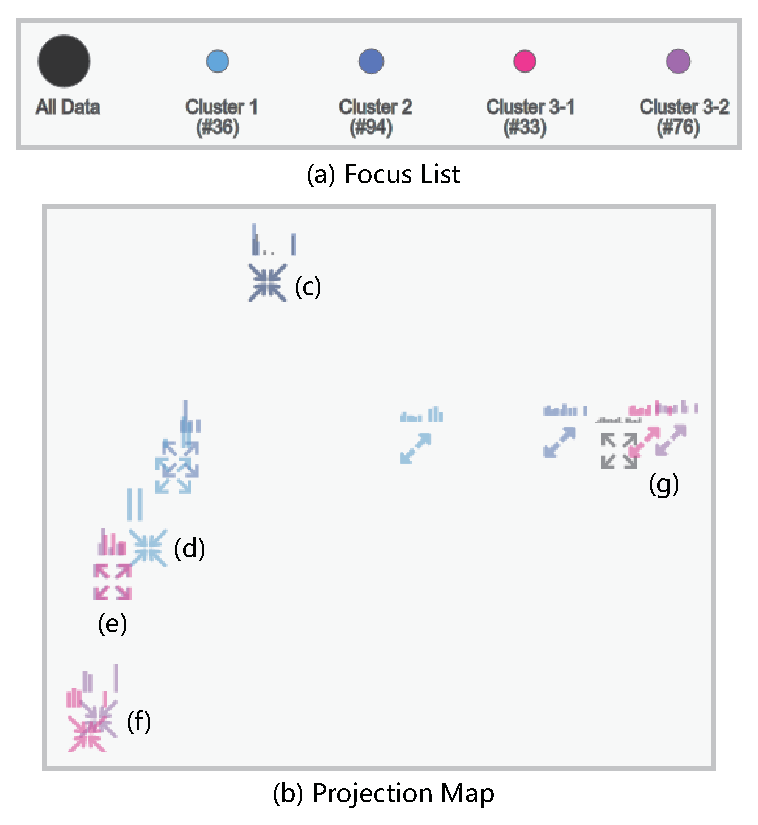
\includegraphics[width=0.85\linewidth]{images/map_1.eps}% 1\linewidth
  \caption{USDA Food Data: we choose a global cluster as the focus, and found outliers }
\label{fig:map}
  \end{figure}

In the above process, we have found outliers and hierarchical clusters in different levels of locality. The four clusters seem layered in the overview(Figure~\ref{fig:food2}(i), (j), Figure~\ref{fig:food3}(g), (h)). Without the featured local projections, it's hard for users to discover and interpret those clusters. Besides, the projections also help to understand the unselected data, and how the focus resembles or differs from them. This will be impossible if the context data are discarded in the projection.

\begin{figure*}[htbp]
\centering
  \includegraphics[width=0.97\linewidth]{images/food_1.eps}% 1\linewidth
  \caption{USDA Food Data: We choose a global cluster as the focus (a), and customize the projection to explore its features (b, c). Outliers can be found in the suggested subspace (d), which are hard to discern in the global projection (f). See Section~\ref{case:food} for more details.}
\label{fig:food1}
  \end{figure*}

\begin{figure*}[htbp]
\centering
  \includegraphics[width=0.97\linewidth]{images/food_2.eps}% 1\linewidth
  \caption{We focus on the cluster found in the subspace (Figure~\ref{fig:food1} (e)). Similarities (b) and diversities (c) are revealed among the cluster members. Three smaller clusters are found. One of them has a strong pattern that it contains no fibers of beta carotene (g). It could be a group of animal-based foods. See Section~\ref{case:food} for more details.}
\label{fig:food2}
  \end{figure*}

\begin{figure*}[htbp]
\centering
  \includegraphics[width=0.97\linewidth]{images/food_3.eps}% 1\linewidth
  \caption{We choose a sub-cluster found in Figure~\ref{food2}(f) to be the new focus. After removing some outliers within the cluster (b), we can see both strong features (d) and interesting inner structures (c) are revealed in the locally enhanced projections. Again, we find two sub-clusters (e, f) within the focus. They seem to be small neighboring clusters in the overview. See Section~\ref{case:food} for more details.}
\label{fig:food3}
  \end{figure*}

\note{compare to histograms: easy to find the most featured dimensions}
\section{Discussion}
\section{Conclusion}

%% if specified like this the section will be committed in review mode
\acknowledgments{
The authors wish to thank A, B, C. This work was supported in part by
a grant from XYZ.}

\bibliographystyle{abbrv}
%%use following if all content of bibtex file should be shown
%\nocite{*}
\bibliography{viewpoingchanger}
\end{document}
